%!Mode:: "TeX:UTF-8"
% !TEX program  = xelatex
\documentclass[a4paper,11pt,UTF8,AutoFakeBold]{ctexart}

% 引入宏定义 macros.tex
% !TeX program = xelatex

\usepackage{indentfirst} %缩进
\usepackage{xeCJK}    %使用系统字体
\usepackage{bm}       %粗体
\usepackage{fancyhdr} %自定义页眉页脚
%\pagestyle{empty}    % 没有页眉页脚
\pagestyle{plain}     % 没有页眉,页脚包含一个居中的页码
\usepackage{amsmath, amsthm, amssymb, amsfonts} %数学公式
\usepackage[a4paper,left=3cm,right=3cm,top=3.5cm,bottom=3.5cm]{geometry}
\usepackage{booktabs} %插入表格
\usepackage[section]{placeins} %避免浮动
\usepackage{listings} %插入代码
\usepackage{underscore} % 在非数学环境下不再需要转义 '_'
\usepackage{ctex}     %中文宏包
\usepackage[svgnames, table]{xcolor} %彩色表格
\usepackage{algorithm}          %伪代码
\usepackage{algorithmicx}
\usepackage{algpseudocode}
\usepackage{algorithm,algpseudocode,float}
\usepackage{lipsum}
\usepackage{enumitem}           %调整列举环境
\usepackage{url}
\usepackage{fontspec,xunicode}
\usepackage{tabularx}            % 增强表格
\usepackage{multirow}            % 多行、多列
\defaultfontfeatures{Mapping=tex-text} %如果没有它,会有一些 tex 特殊字符无法正常使用,比如连字符。
\usepackage[explicit]{titlesec}
\usepackage[breaklinks,colorlinks,linkcolor=black,citecolor=black,urlcolor=black]{hyperref} % 生成 PDF 书签
\usepackage{float}
\usepackage{xifthen} % provides \isempty test



\usepackage{graphicx}
\graphicspath{{imgs/}}

%%%%%%%%%%%%%%%%%%%%%%%%%%%%%%%%%%%%%%%%%%%%%%%%%%%%%%%%%%%%%%%%
% 缩进及行间距
%%%%%%%%%%%%%%%%%%%%%%%%%%%%%%%%%%%%%%%%%%%%%%%%%%%%%%%%%%%%%%%%
\setlength{\parindent}{22bp} %重新定义缩进长度
\linespread{1}

%%%%%%%%%%%%%%%%%%%%%%%%%%%%%%%%%%%%%%%%%%%%%%%%%%%%%%%%%%%%%%%%
% 图的标题行间距设置
%%%%%%%%%%%%%%%%%%%%%%%%%%%%%%%%%%%%%%%%%%%%%%%%%%%%%%%%%%%%%%%%
\newcommand{\bottomcaption}{%
    \setlength{\abovecaptionskip}{6bp}%
    \setlength{\belowcaptionskip}{6bp}%
    \caption
}

%%%%%%%%%%%%%%%%%%%%%%%%%%%%%%%%%%%%%%%%%%%%%%%%%%%%%%%%%%%%%%%%
% 字体定义
%%%%%%%%%%%%%%%%%%%%%%%%%%%%%%%%%%%%%%%%%%%%%%%%%%%%%%%%%%%%%%%%
\setmainfont{Times New Roman}  %默认英文字体.serif是有衬线字体sans serif无衬线字体
\setmonofont{Consolas}
\setCJKmainfont[ItalicFont={宋体}, BoldFont={黑体}]{宋体}%衬线字体 缺省中文字体为 
% \punctstyle{hangmobanjiao}
%-----------------------xeCJK下设置中文字体------------------------------%
\setCJKfamilyfont{song}{SimSun}                             %宋体 song
\newcommand{\song}{\CJKfamily{song}}
\setCJKfamilyfont{fs}{FangSong}                      %仿宋  fs
\newcommand{\fs}{\CJKfamily{fs}}
\let\kaishu\relax                                    %重定义楷体,打开假粗体
\newCJKfontfamily\kaishu{KaiTi}[AutoFakeBold]
%\setCJKfamilyfont{ktgb}{KaiTi_GB2312}                      %楷体 GB2312
%\newcommand{\ktgb}{\CJKfamily{ktgb}}
\setCJKfamilyfont{yh}{Microsoft YaHei}                    %微软雅黑 yh
\newcommand{\yh}{\CJKfamily{yh}}
\setCJKfamilyfont{hei}{SimHei}                              %黑体  hei
\newcommand{\hei}{\CJKfamily{hei}}
\setCJKfamilyfont{hwxk}{STXingkai}                                %华文行楷  hwxk
\newcommand{\hwxk}{\CJKfamily{hwxk}}
\setCJKfamilyfont{fzshu}{FZShuTi}                                    %方正舒体 fzshu
\newcommand{\fzshu}{\CJKfamily{fzshu}}
%------------------------------设置字体大小------------------------%
\newcommand{\chuhao}{\fontsize{42bp}{63bp}\selectfont}     %初号, 1.5倍行距
\newcommand{\xiaochuhao}{\fontsize{36bp}{36bp}\selectfont} %小初号,单倍行距
\newcommand{\yihao}{\fontsize{26bp}{39bp}\selectfont}        % 一号, 1.5 倍行距
\newcommand{\erhao}{\fontsize{22bp}{33bp}\selectfont}        % 二号, 1.5倍行距
\newcommand{\xiaoerhao}{\fontsize{18bp}{18bp}\selectfont}       % 小二, 单倍行距
\newcommand{\sanhao}{\fontsize{16bp}{24bp}\selectfont}       % 三号, 1.5倍行距
\newcommand{\xiaosanhao}{\fontsize{15bp}{22bp}\selectfont}      % 小三, 1.5倍行距
\newcommand{\sihao}{\fontsize{14bp}{21bp}\selectfont}        % 四号, 1.5 倍行距
\newcommand{\banxiaosi}{\fontsize{13bp}{20bp}\selectfont}  % 半小四, 20pt行距
\newcommand{\xiaosihao}{\fontsize{12bp}{20bp}\selectfont}       % 小四, 20pt行距
\newcommand{\dawuhao}{\fontsize{11bp}{11bp}\selectfont}      % 大五号, 单倍行距
\newcommand{\wuhao}{\fontsize{10.5bp}{10.5bp}\selectfont}   % 五号, 单倍行距
\newcommand{\xiaowuhao}{\fontsize{9bp}{9bp}\selectfont}   %小五号,单倍行距
%------------------------------重定义normalize------------------------%
\renewcommand{\normalsize}{\fontsize{12bp}{20bp}\selectfont}


%%%%%%%%%%%%%%%%%%%%%%%%%%%%%%%%%%%%%%%%%%%%%%%%%%%%%%%%%%%%%%%%
% 图题字体大小相同
%%%%%%%%%%%%%%%%%%%%%%%%%%%%%%%%%%%%%%%%%%%%%%%%%%%%%%%%%%%%%%%%
\usepackage{caption}
\captionsetup{font={footnotesize}}   % footnotesize = 9bp
\captionsetup[lstlisting]{font={footnotesize}}

%%%%%%%%%%%%%%%%%%%%%%%%%%%%%%%%%%%%%%%%%%%%%%%%%%%%%%%%%%%%%%%%
% 重定义枚举编号为 1),2)...
%%%%%%%%%%%%%%%%%%%%%%%%%%%%%%%%%%%%%%%%%%%%%%%%%%%%%%%%%%%%%%%%
\renewcommand{\labelenumi}{\theenumi)}


%%%%%%%%%%%%%%%%%%%%%%%%%%%%%%%%%%%%%%%%%%%%%%%%%%%%%%%%%%%%%%%%
% 重定义section标题
%%%%%%%%%%%%%%%%%%%%%%%%%%%%%%%%%%%%%%%%%%%%%%%%%%%%%%%%%%%%%%%%
\CTEXsetup[format={\song\bfseries\zihao{4}},number={\chinese{section}},name={,、~},aftername={},indent={0bp},beforeskip={6bp},afterskip={6bp},format+={\flushleft}]{section}
\CTEXsetup[format={\Large\bfseries\song\zihao{5}},name={(,)},number={\chinese{subsection}},aftername={},indent={22bp},beforeskip={6bp},afterskip={6bp}]{subsection}
\CTEXsetup[format={\Large\bfseries\song\zihao{5}},name={,.},aftername={ },indent={28bp},beforeskip={6bp},afterskip={6bp}]{subsubsection}
\CTEXsetup[number={\chinese{section}},name={附录, ~~ }]{appendix}



%%%%%%%%%%%%%%%%%%%%%%%%%%%%%%%%%%%%%%%%%%%%%%%%%%%%%%%%%%%%%%%%
% 标题名称中文化
%%%%%%%%%%%%%%%%%%%%%%%%%%%%%%%%%%%%%%%%%%%%%%%%%%%%%%%%%%%%%%%%
\renewcommand\figurename{\hei 图}
\renewcommand\tablename{\hei 表}
\renewcommand\lstlistingname{\hei 代码}
\renewcommand{\algorithmicrequire}{\textbf{输入:}}
\renewcommand{\algorithmicensure}{\textbf{输出:}}
\newtheorem{define}{定义}


%%%%%%%%%%%%%%%%%%%%%%%%%%%%%%%%%%%%%%%%%%%%%%%%%%%%%%%%%%%%%%%%
% 列表设置
%%%%%%%%%%%%%%%%%%%%%%%%%%%%%%%%%%%%%%%%%%%%%%%%%%%%%%%%%%%%%%%%
\setlist[enumerate,1]{leftmargin=46bp,listparindent=0bp,itemsep=0mm,partopsep=.7mm,parsep=0ex,labelsep=1.5mm,topsep=0.7mm}
\setlist[enumerate,2]{label=\alph*),leftmargin=1.5em}  %二级item设置
\setitemize{leftmargin=46bp,listparindent=0bp,itemsep=0mm,partopsep=.7mm,parsep=0ex,labelsep=1.5mm,topsep=0.7mm}
\setitemize{itemindent=38bp,leftmargin=0bp,itemsep=-0.4ex,listparindent=26bp,partopsep=0bp,parsep=0.5ex,topsep=-0.25ex}
%\setdescription{itemindent=38bp,leftmargin=0bp,itemsep=-0.4ex,listparindent=26bp,partopsep=0bp,parsep=0.5ex,topsep=-0.25ex}

%%%%%%%%%%%%%%%%%%%%%%%%%%%%%%%%%%%%%%%%%%%%%%%%%%%%%%%%%%%%%%%%
% 代码设置
%%%%%%%%%%%%%%%%%%%%%%%%%%%%%%%%%%%%%%%%%%%%%%%%%%%%%%%%%%%%%%%%
\lstset{
 columns=fixed,
 numbers=left,                                        % 在左侧显示行号
 numberstyle=\tiny\color{gray},                       % 设定行号格式
 frame=single,                                        % 单线背景边框
 breaklines=true,                                     % 设定LaTeX对过长的代码行进行自动换行
 keywordstyle=\color[RGB]{40,40,255},                 % 设定关键字颜色
 numberstyle=\footnotesize\color{darkgray},
 commentstyle=\it\color[RGB]{0,96,96},                % 设置代码注释的格式
 stringstyle=\rmfamily\slshape\color[RGB]{128,0,0},   % 设置字符串格式
 showstringspaces=false,                              % 不显示字符串中的空格
 language=java,                                        % 设置语言
 basicstyle=\linespread{1.0}\xiaowuhao\ttfamily,                      % 字体字号
 %lineskip=10bp,
 %baselinestretch=1,
}


%%%%%%%%%%%%%%%%%%%%%%%%%%%%%%%%%%%%%%%%%%%%%%%%%%%%%%%%%%%%%%%%
% 伪代码分页
%%%%%%%%%%%%%%%%%%%%%%%%%%%%%%%%%%%%%%%%%%%%%%%%%%%%%%%%%%%%%%%%
\makeatletter
\renewcommand{\ALG@name}{算法}
\newenvironment{breakablealgorithm}
  {% \begin{breakablealgorithm}
   \begin{center}
     \refstepcounter{algorithm}% New algorithm
     \hrule height.8bp depth0bp \kern2bp% \@fs@pre for \@fs@ruled
     \renewcommand{\caption}[2][\relax]{% Make a new \caption
       {\raggedright\textbf{\ALG@name~\thealgorithm} ##2\par}%
       \ifx\relax##1\relax % #1 is \relax
         \addcontentsline{loa}{algorithm}{\protect\numberline{\thealgorithm}##2}%
       \else % #1 is not \relax
         \addcontentsline{loa}{algorithm}{\protect\numberline{\thealgorithm}##1}%
       \fi
       \kern2bp\hrule\kern2bp
     }
  }{% \end{breakablealgorithm}
     \kern2bp\hrule\relax% \@fs@post for \@fs@ruled
   \end{center}
  }
\makeatother


%%%%%%%%%%%%%%%%%%%%%%%%%%%%%%%%%%%%%%%%%%%%%%%%%%%%%%%%%%%%%%%%
% 设置 \part
%%%%%%%%%%%%%%%%%%%%%%%%%%%%%%%%%%%%%%%%%%%%%%%%%%%%%%%%%%%%%%%%

\titleformat{\part}[display]{}{}{0pt}{}
%\titlespacing*{\part}{0pt}{0pt}{0pt}   % 在正文中隐藏 part
\makeatletter
\@addtoreset{section}{part} % 使 section 在 part 后重新标号
\makeatother


%%%%%%%%%%%%%%%%%%%%%%%%%%%%%%%%%%%%%%%%%%%%%%%%%%%%%%%%%%%%%%%%
% 设置个人信息
%%%%%%%%%%%%%%%%%%%%%%%%%%%%%%%%%%%%%%%%%%%%%%%%%%%%%%%%%%%%%%%%
\makeatletter
\newcommand{\course}[1]{
    \newcommand{\report@course}{#1}
}
\newcommand{\college}[1]{
    \newcommand{\report@college}{#1}
}
\newcommand{\major}[1]{
    \newcommand{\report@major}{#1}
}
\newcommand{\studentid}[1]{
    \newcommand{\report@studentid}{#1}
}
%\newcommand{\theauthor}[1]{
%    \newcommand{\report@author}{#1}
%}
\newcommand{\teacher}[1]{
    \newcommand{\report@teacher}{#1}
}
\newcommand{\thedate}[1]{
    \newcommand{\report@date}{#1}
}
\makeatother


%%%%%%%%%%%%%%%%%%%%%%%%%%%%%%%%%%%%%%%%%%%%%%%%%%%%%%%%%%%%%%%%
% 设置 \maketitle
%%%%%%%%%%%%%%%%%%%%%%%%%%%%%%%%%%%%%%%%%%%%%%%%%%%%%%%%%%%%%%%%
\makeatletter
\renewcommand{\maketitle}{
    \thispagestyle{empty}   % 去掉首页页码
    \begin{titlepage}

        \begin{figure}[!htbp]
            \centering
            
\includegraphics[width=\textwidth]{uestc}
        \end{figure}

        \center{\xiaochuhao{\kaishu 计算机专业类课程}}
        \vspace{1.5cm}
        \center{\fontsize{48bp}{52bp}{\song{\bfseries 实\\验\\报\\告}}}

        \vspace{1.5cm}

        \begin{center}
            \begin{large}
                \begin{tabular}{rl}
                    \xiaoerhao{\bfseries\fs{课程名称:}}& \xiaoerhao{\bfseries\hei{\report@course}}\\
                    \\
                    \xiaoerhao{\bfseries\fs{学\qquad 院:}}& \xiaoerhao{\bfseries\hei{\report@college}}\\
                    \\
                    \xiaoerhao{\bfseries\fs{学院专业:}}& \xiaoerhao{\bfseries\hei{\report@major}}\\
                    \\
                    \xiaoerhao{\bfseries\fs{学\qquad 号:}}& \xiaoerhao{\bfseries\hei{\report@studentid}}\\
                    \\
                    \xiaoerhao{\bfseries\fs{学生姓名:}}& \xiaoerhao{\bfseries\hei{\@author}}\\
                    \\
                    \xiaoerhao{\bfseries\fs{指导教师:}}& \xiaoerhao{\bfseries\hei{\report@teacher}}\\
                    \\
                    \xiaoerhao{\bfseries\fs{日\qquad 期:}}& \xiaoerhao{\bfseries\hei{\report@date}}\\
                \end{tabular}
            \end{large}
        \end{center}
    \end{titlepage}
    \newpage
    \setcounter{page}{1} % 第二页从 1 开始标号
}
\makeatother

%%%%%%%%%%%%%%%%%%%%%%%%%%%%%%%%%%%%%%%%%%%%%%%%%%%%%%%%%%%%%%%%
% 设置 \chapter
%%%%%%%%%%%%%%%%%%%%%%%%%%%%%%%%%%%%%%%%%%%%%%%%%%%%%%%%%%%%%%%%

\makeatletter
\newcommand{\chapter}[3]{
    \newpage
    \part{}
    \vspace*{-120bp} % Adjust the vertical space here
    \centerline{\\[40bp]\erhao{\fzshu{\bfseries 电 ~子 ~科~ 技~ 大~ 学}}}
    \vspace*{-20bp} % Adjust the vertical space her
    \centerline{\\[20bp]\yihao{\hei{\bfseries 实  ~~~ 验  ~~~ 报  ~~~ 告}}}

    \ifthenelse{\isempty{#3}}{
        \centerline{\\[20bp]\yihao{\song{\bfseries #1}}}
    }{
        \noindent
        \begin{tabularx}{\textwidth}{XXX}
            \Large\bfseries\song\zihao{4}学生姓名:{\@author} &
            \Large\bfseries\song\zihao{4}学 号:{\report@studentid} &
            \Large\bfseries\song\zihao{4}指导教师:{\report@teacher}
        \end{tabularx}\\

        \noindent
        \begin{tabularx}{\textwidth}{XX}
            \Large\bfseries\song\zihao{4}实验地点:{#2} &
            \Large\bfseries\song\zihao{4}实验时间:{#3}
        \end{tabularx}
    }
}
\makeatother



\begin{document}
\xiaosihao \setCJKfamilyfont{song}{SimSun}  

\course{计算机视觉与模式识别}
\college{计算机科学与工程学院}
\major{计算机科学与技术}
\studentid{2022010910017}
\author{谢卿云}
\teacher{沈复民}
\thedate{2025 年 5 月 10 日}

% \maketitle

%\chapter{实验一}{}{}                                      % 用于单次实验报告开头的 “实验X”
\chapter{}{}{}           % 实验信息

\section{实验项目名称:}
Scene Recognition with Bag of Words

\section{实验原理:}
\subsection{Tiny Images 实验原理}

Tiny Images 是一种简单而有效的图像特征表示方法,
其核心思想是将高分辨率图像缩放到小尺寸,
并将像素值展平作为特征向量。
Tiny Images常常在场景识别任务中作为基准方法或与其他特征结合使用时,
仍能取得一定的效果。
在本实验中,将Tiny Images与KNN分类器结合,
作为探索不同特征和分类器组合的第一步。

\subsubsection{方法特点}
Tiny Images方法具有以下特点:

\begin{itemize}
    \item \textbf{计算效率高}:特征提取过程简单快速
    \item \textbf{低维表示}:特征向量维度较低(如256维)
    \item \textbf{全局特征}:捕捉图像的整体低频信息
    \item \textbf{对细节不敏感}:对噪声和细节变化具有鲁棒性
    \item \textbf{对几何变换敏感}:对图像的平移、旋转和缩放敏感
\end{itemize}

\subsubsection{基本原理}
Tiny Images 方法通过以下步骤将图像转换为特征向量:

\begin{enumerate}
    \item \textbf{图像缩放}:将原始图像强制缩放到固定的小尺寸(如16x16像素),保留整体结构信息。
    
    \item \textbf{灰度转换}:将彩色图像转换为灰度图像,简化特征表示。
    
    \item \textbf{特征向量生成}:将缩放后的图像像素值按序排列,形成一维特征向量。对于16x16的灰度图像,得到256维向量。
    
    \item \textbf{特征归一化}:对特征向量进行归一化处理,减少光照等因素的影响。
\end{enumerate}
\section{K近邻分类器实验原理}

K近邻(K-Nearest Neighbors, KNN)是一种简单直观的监督学习算法,
主要用于分类和回归任务。
在本实验中,它被用作分类器,特别是与Tiny Images特征结合使用。

\subsection{基本原理}
KNN的核心思想是:一个样本的类别由其在特征空间中的K个最近邻居的类别决定。

\subsection{KNN特点}
\begin{itemize}
    \item \textbf{简单易懂}:原理直观,易于实现
    \item \textbf{无需训练}:仅存储训练数据,无复杂训练过程
    \item \textbf{计算开销}:预测阶段需计算与所有训练样本的距离,大数据集上耗时
    \item \textbf{对噪声敏感}:K值较小时对噪声和离群点敏感
    \item \textbf{维数灾难}:高维特征空间中距离计算意义减弱,数据稀疏
    \item \textbf{非参数模型}:不对数据分布做假设
\end{itemize}

\subsection{算法步骤}
算法流程如下伪代码所示
\begin{algorithm}[H]
  \caption{Pseudocode for K-Nearest Neighbors (KNN) Classification}
  \begin{algorithmic}[1]
    \Require Test data feature vector $x_{\text{test}}$,Training data feature vectors $\text{TrainingData} = \{x_1, x_2, ..., x_n\}$,Corresponding training labels $\text{TrainingLabels} = \{y_1, y_2, ..., y_n\}$,Number of nearest neighbors $K$
    \Ensure Predicted class label $y_{\text{pred}}$ for $x_{\text{test}}$
    \State Initialize an empty list: $\text{NeighborsList}$ (to store Distance, Label tuples)

    \For{each training sample $x_i$ in $\text{TrainingData}$}
      \State Calculate the distance between $x_{\text{test}}$ and $x_i$: $Distance_i \leftarrow \text{Distance}(x_{\text{test}}, x_i)$
      \State Get the corresponding label $y_i$ from $\text{TrainingLabels}$
      \State Add tuple $(Distance_i, y_i)$ to $\text{NeighborsList}$
    \EndFor

    \State Sort $\text{NeighborsList}$ based on distance in ascending order

    \State Select the first $K$ elements from sorted $\text{NeighborsList}$ as $\text{K\_Nearest\_Neighbors}$

    \State Initialize an empty map: $\text{LabelCounts}$ (to count frequency of labels)

    \For{each neighbor $(distance, label)$ in $\text{K\_Nearest\_Neighbors}$}
      \State Increment count for $\text{label}$ in $\text{LabelCounts}$
    \EndFor

    \State Find the label with the maximum count in $\text{LabelCounts}$
    \State $y_{\text{pred}} \leftarrow \text{Label with highest count in } \text{LabelCounts}$
    \Comment{Handle ties if necessary}

    \State \Return $y_{\text{pred}}$
  \end{algorithmic}
\end{algorithm}


\subsection{K值选择}
参数K是KNN算法最重要的决定因素:
\begin{itemize}
    \item K=1时,新样本类别由最近训练样本决定,对噪声敏感
    \item 增大K可减少噪声影响,使决策边界更平滑
    \item K过大可能包含不相关邻居,导致性能下降
    \item 通常通过交叉验证选择最优K值
\end{itemize}




\subsection{Bag of Words (BoW) 实验原理}

Bag of Words (BoW) 模型最初用于文本分析,
将文档表示为其包含的单词的频率直方图,忽略词语的顺序。
将这个思想迁移到图像领域,就是将图像视为"视觉词汇"的集合。
BoW模型通过提取局部特征、构建视觉词汇表、生成特征直方图等步骤,
实现了对图像内容的有效表示。这种方法能够捕捉图像中具有辨识度的局部信息,
在许多图像分类任务中取得了不错的性能。
在本实验中,我们使用SIFT特征实现对场景的分类;

\subsubsection{基本原理}
BoW模型通过以下步骤将图像转换为特征向量:

\begin{enumerate}
    \item \textbf{局部特征提取}:
    使用SIFT算法检测图像中的关键点,
    计算每个关键点的128维特征描述符。
    特征描述符对尺度和旋转变换具有鲁棒性。
    
    \item \textbf{构建视觉词汇表}:
    收集所有训练图像的SIFT特征描述符,
    使用K-Means聚类算法构建视觉词汇表。
    每个聚类中心代表一个视觉词汇,
    词汇表大小(vocab\_size)需要预先设定。
    
    \item \textbf{特征向量生成}:
    对每张图像提取SIFT特征,
    将特征映射到最近的视觉词汇,
    统计每个视觉词汇的出现频率,
    生成vocab\_size维的直方图特征向量。
    
    \item \textbf{分类}:
    使用SVM等分类器进行训练和预测,
    学习特征向量与图像类别的关系。
\end{enumerate}


\subsection{支持向量机 (SVM) 实验原理}

支持向量机 (Support Vector Machine, SVM) 是一种强大的监督学习模型,
主要用于分类和回归任务。在本次场景分类实验中,
我们将使用 SVM 作为 Bag of Words 特征的分类器。

SVM 的核心思想是寻找一个最优的超平面 (Hyperplane) 来在高维特征空间中将不同类别的样本分开。
这个最优超平面不仅要能正确划分样本,
还要使两类样本中的支持向量到超平面的间隔(Margin)最大化。
最大化间隔可以提高分类器的泛化能力,使其在新数据上表现更好。

\subsubsection{数学原理}

对于一个二分类问题,给定一组带有标签的训练数据,SVM 的目标是找到一个决策函数,通常是线性的:
    \[ f(\mathbf{x}) = \mathbf{w} \cdot \mathbf{x} + b \]
其中 \(\mathbf{w}\) 是超平面的法向量,\(b\) 是偏置项。超平面由 \(\mathbf{w} \cdot \mathbf{x} + b = 0\) 定义。

对于训练样本 \((x_i, y_i)\),
其中 \(x_i\) 是特征向量,
\(y_i \in \{-1, 1\}\) 是类别标签,
我们希望找到 \(\mathbf{w}\) 和 \(b\),使得:
    \[ y_i (\mathbf{w} \cdot x_i + b) \ge 1 \]
同时,我们希望最小化 \(\|\mathbf{w}\|^2\),
等价于最大化间隔 \(2/\|\mathbf{w}\|\)),
这是一个凸优化问题,可以通过拉格朗日乘子法等技术求解。

在实际应用中,数据往往不是完全线性可分的。
SVM 引入了\textbf{软间隔 (Soft Margin)} 的概念,
允许少量样本点违反间隔约束,
即允许一些样本点位于间隔带内甚至错误的一侧。
这通过引入松弛变量 \(\xi_i \ge 0\) 和惩罚参数 \(C\) 来实现,优化目标变为最小化:
    \[ \frac{1}{2}\|\mathbf{w}\|^2 + C \sum_{i=1}^n \xi_i \]
约束条件变为:
\[ y_i (\mathbf{w} \cdot x_i + b) \ge 1 - \xi_i \]

\subsubsection{Kernel Trick}

对于非线性可分的数据,SVM 使用\textbf{核技巧 (Kernel Trick)} 
将原始特征空间映射到更高维的空间,
使得样本在该高维空间中变得线性可分。
常用的核函数包括多项式核、径向基函数 (RBF) 核等。核函数 \(K(\mathbf{x}_i, \mathbf{x}_j)\) 计算的是样本在映射后的高维空间中的内积,而无需显式计算高维映射本身,这大大提高了计算效率。

然而,在本次实验中,由于使用了 `sklearn.svm.LinearSVC`,
这表示我们主要考虑线性分类器,
或者等价于使用了线性核 
    \(K(\mathbf{x}_i, \mathbf{x}_j) = \mathbf{x}_i \cdot \mathbf{x}_j\)。
线性 SVM 在处理高维稀疏数据时通常非常高效,这与 Bag of Words 特征的特性相符。

\subsubsection{多类别分类}

SVM 本身是二分类器。对于像场景分类这样的多类别任务(假设有 M 个类别),
需要将二分类 SVM 扩展。常用的策略有两种:

\begin{enumerate}
    \item \textbf{一对多 (One-vs-Rest, OvR):} 为每个类别训练一个二分类 SVM。例如,对于类别 k,训练一个分类器来区分类别 k 的样本和所有非类别 k 的样本。总共需要训练 M 个分类器。在预测时,将待分类样本输入所有 M 个分类器,选择输出分数最高(或离超平面最远)的那个类别作为预测结果。`LinearSVC` 默认通常采用 One-vs-Rest 策略。
    \item \textbf{一对一 (One-vs-One, OvO):} 为每一对不同的类别训练一个二分类 SVM。例如,对于类别 i 和类别 j,训练一个分类器来区分这两类样本。总共需要训练 \(M(M-1)/2\) 个分类器。在预测时,将待分类样本输入所有分类器,然后使用投票机制决定最终类别。每个分类器都为其中一个类别投一票,得票最多的类别获胜。
\end{enumerate}
在本次实验中,我们使用的 `LinearSVC` 通常采用 One-vs-Rest 策略来实现多类别分类。
% \subsection{DNN原理}

在传统的图像分类方法中,特征提取(如 Tiny Images, SIFT+BoW)和分类是分开进行的两个步骤。而深度神经网络 (DNN),尤其是卷积神经网络 (CNN),能够将特征学习和分类集成到一个端到端的模型中,通过多层非线性变换自动从原始像素数据中学习到具有判别力的层次化特征。

\subsubsection{深度神经网络 (DNN) 原理}

深度神经网络由多个层组成,每一层都对输入进行某种变换,
并将结果传递给下一层。通过堆叠多层,
网络能够学习越来越抽象和复杂的特征表示。
对于图像任务,\textbf{卷积神经网络 (CNN)} 是最成功的 DNN 架构。
CNN 的核心在于其能够有效地处理具有网格状拓扑结构的数据(如图像)。

一个典型的 CNN 架构通常包含以下几种类型的层:

\begin{itemize}
    \item \textbf{卷积层 (Convolutional Layer):} 通过一组可学习的滤波器对输入图像进行卷积操作,提取局部特征。每个滤波器学习一种特定的空间模式。卷积操作通过权值共享和利用图像的空间局部相关性减少参数数量。
    \item \textbf{激活函数层 (Activation Layer):} 在卷积操作之后,应用非线性激活函数(如 ReLU)。非线性是学习复杂模式的关键。
    \item \textbf{池化层 (Pooling Layer):} 用于减小特征图的空间尺寸,同时保留重要信息。常见的有最大池化和平均池化,提供平移不变性。
    \item \textbf{全连接层 (Fully Connected Layer):} 将高级特征映射到最终的输出(如类别得分)。每个神经元与前一层的所有神经元相连。
    \item \textbf{输出层 (Output Layer):} 最后一层,通常结合 Softmax 转换为类别概率分布。
\end{itemize}

\subsubsection{PyTorch框架部署DNN}

PyTorch 提供了构建、训练和部署 DNN 模型的灵活工具。
在 PyTorch 中实现基于 CNN 的场景分类任务,通常遵循以下流程:
通过 PyTorch,我们可以灵活地定义复杂的 CNN 结构,
利用其自动求导机制进行高效训练,并方便地在 GPU 上加速计算。


\section{实验目的:}
\begin{enumerate}
    \item 理解并实践不同的图像全局特征和局部特征的提取与表示方法。
    \item 学习并应用 K 近邻 (KNN) 和 支持向量机 (SVM) 等经典分类器在图像识别任务中的原理和使用。
    \item 通过比较不同特征和不同分类器组合的分类性能,分析它们对最终结果的影响。
    \item 初步了解并实现基于深度神经网络 (DNN) 的场景分类方法,体验其与传统方法的差异。
    \item 掌握评估分类模型性能的方法,并能够对实验结果进行分析和讨论,总结不同方法的优劣和适用场景。
\end{enumerate}


\section{实验内容:}
\begin{enumerate}
	\item 分别利用 Tiny+KNN 和 Bags of Words (SIFT) + SVM 实现对场景的分类,并且比较不同特征和不同分类方法对最终精度的影响;
	\item 用深度神经网络DNN进一步完成场景分类任务,对比其性能。
\end{enumerate}

% \section{实验器材(设备、元器件):}
% Cargo等rust语言包,Linux服务器等

\section{实验步骤:}
\subsection{实现Tiny+KNN方法}
	\begin{enumerate}
		\item 实现student.py/get_tiny_images(image_paths)函数: 
		根据Tiny Images和KNN的实验原理,为输入的图像路径列表生成 Tiny Images 特征。
		输出一个 n x d的 NumPy数组,
		其中 n是图像数量,
		d是 Tiny Images 特征向量的长度(例如 16*16=256);

		\item 完善 `nearest_neighbor_classify(train_image_feats, train_labels, test_image_feats)` 函数
		使用 KNN 分类器对测试图像进行分类。
		为输入的图像路径列表生成 Tiny Images 特征。
		输出一个 n x d的 NumPy数组,
		其中 n是图像数量,
		d是 Tiny Images 特征向量的长度(例如 16*16=256);
		输出一个m x 1的 NumPy 数组,
		其中m是测试图像数量,每个元素是对应的预测类别标签。

	\end{enumerate}


\subsection{实现 Bag of Words (SIFT) + SVM 方法}
	\begin{enumerate}
		\item 实现student.py/build_vocabulary(image_paths, vocab_size)函数
		根据Bag of Words (SIFT) + SVM的实验原理,
		从训练图像中提取 HOG 特征并构建视觉词汇,
		输出一个vocab_size x (z*z*9)的 NumPy 数组,
		代表聚类中心(即视觉词汇)。
		通常会将这个词汇保存到文件vocab.npy。

		\item 实现 get_bags_of_words(image_paths)函数,
		为输入的图像路径列表生成 Bag of Words 直方图特征,
		加载已构建的视觉词汇 (vocab.npy),
		输出一个n x vocab_size的 NumPy 数组,
		其中n是图像数量,vocab_size是词汇大小,
		每个元素是对应的 Bag of Words 直方图特征向量。

		\item 完善 svm_classify(train_image_feats, train_labels, test_image_feats)函数;
		使用 SVM 分类器对测试图像进行分类
		输出一个m x 1的 NumPy 数组,
		其中m是测试图像数量,
		每个元素是对应的预测类别标签。
	\end{enumerate}


\subsection{实现 DNN 网络}
在proj4.ipynb重新开一个单元格,用于实现DNN

\subsection{比较分析}
	\begin{enumerate}
		\item 在完成以上实现后,运行proj4.ipynb所有单元格。
		\item 计算 Tiny+KNN、BoW+SVM 和 DNN在测试集上的分类精度。
		\item 比较这三种方法的精度,分析不同特征表示和不同分类器对场景分类性能的影响。
	\end{enumerate}
    

\section{实验数据及结果分析:}
运行第一组(Tiny+KNN)的结果如图1所示,
\begin{figure}[hbt!]
    \centering
    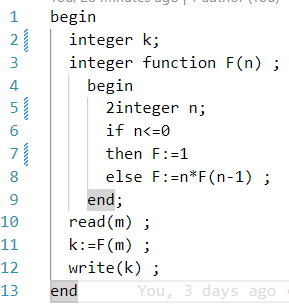
\includegraphics[width=0.8\textwidth]{imgs/1.png} % 确保图片文件路径正确
    \caption{Tiny Image + KNN 混淆矩阵}
    \label{图1:}
\end{figure}
可以看到整体准确率仅有0.189,接近随机猜测(理论上15类随机猜测准确率为1/15 ≈ 0.067)。

运行第二组(Bags of Words + SVM)的结果如图2所示,
\begin{figure}[hbt!]
    \centering
    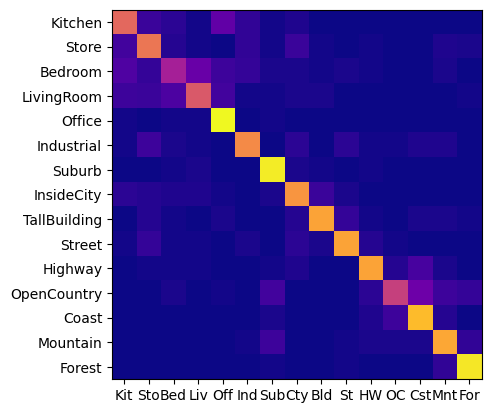
\includegraphics[width=0.8\textwidth]{imgs/2.png} % 确保图片文件路径正确
    \caption{Bag of Words + SVM 混淆矩阵}
    \label{图2:}
\end{figure}
整体准确率上升至0.711,显著高于第一组。


\section{实验结论:}
实验结果显示,第二种方法(BOW + SVM)的准确率
远高于第一种方法(Tiny Image + KNN)的准确率。
推测原因如下:

Tiny Image 特征是非常简单的全局特征,仅通过将图片缩放到非常小的尺寸来表示。
这种方法丢失了图像的绝大部分细节信息,对图像的尺度、平移、旋转以及视角变化非常敏感。
它只能捕获非常粗略的空间布局和颜色信息,难以区分细节丰富的不同场景。
Bags of Words 特征是基于局部特征描述符(如 HOG 或 SIFT)构建的。
这些局部描述符(如 SIFT)能够捕捉图像中具有区分性的局部模式
(如边缘、角点、纹理等),并且对局部的光照、尺度和旋转变化具有一定的鲁棒性。
将这些局部特征聚类形成"视觉词汇",并将图像表示为这些视觉词汇的直方图,
能够更有效地捕获场景的构成元素及其分布,
从而提供了比 Tiny Image 更丰富、更具判别力的图像表示。


KNN分类器是一种基于实例的学习方法,
它直接根据测试样本与训练样本在特征空间中的距离进行分类。
虽然简单直观,但 KNN 对噪声和不相关的特征比较敏感,
并且在处理高维稀疏数据(如 Bag of Words 直方图)时,
"距离"的定义和计算可能会受到"维度灾难"的影响,性能可能受限。
SVM是一种功能强大的分类器,
尤其擅长处理高维数据。
SVM 尝试在特征空间中找到一个最优的超平面来最大化不同类别之间的间隔。
线性 SVM(LinearSVC)虽然是线性的,
但它在高维空间中表现良好,并且通过合适的正则化可以有效地防止过拟合。
相比于 KNN 仅依赖局部少数样本,SVM 学习的是一个全局的决策边界,
这通常在高维复杂的特征空间中更具优势。

综上所述,Bags of Words 方法通过更鲁棒、
更具判别力的局部特征表示捕获了场景的关键信息,
而 SVM 分类器则能够有效地利用这种高维特征进行分类。
因此,BOW + SVM 的组合在场景分类任务上取得了显著优于 Tiny Image + KNN 方法的性能。


\section{总结及心得体会:}
尽管实验成功验证了核心原理并构建了基本框架,但也认识到当前实现作为生产级编译器前端存在诸多不足(如错误恢复的健壮性、符号表中信息的完整性、对复杂文法结构的处理能力、性能优化以及与现代编译器架构的差距等)。

总而言之,本次实验通过从零开始实现一个简单的编译器前端,不仅成功地将编译原理的理论知识转化为实际代码。 通过构建了一个可工作的简单demo,我加深了对词法分析、语法分析、作用域管理和符号表工作原理的理解。实验结果证明了所采用方法的有效性。

\section{对本实验过程及方法、手段的改进建议及展望:}
错误恢复机制 :本项目的词法分析器在遇到非法字符或错误时,会跳过当前行的剩余部分并返回错误。这是一种简单的恐慌模式错误恢复策略,即在检测到错误后,跳过一部分输入直到找到一个看似可以继续解析的同步点。可以设计更加用户友好的错误报告,比如“在 X 处期望得到 Y,但找到了 Z”,并给出可能的修正建议。还比如不仅仅跳到行尾,而是跳到更合适的同步词法单元,例如语句结束符 ;、块的开始/结束符号 (begin, end) 或文件末尾。这需要在文法中定义哪些词法单元可以作为同步点。

目前,对于变量声明的情况,无法维护其所属的过程名。在支持嵌套函数或过程的语言中,一个变量的完全限定名或用于查找作用域链的信息通常需要包含其所在的函数/过程信息。 在解析函数体或任何可能包含变量声明的块时,可以将当前正在解析的函数/过程的名称作为参数传递给其他方法,限于时间有限无法完成。

在文法中没有区分实参和形参,导致进一步语义分析可能出现了意料不到的错误。函数定义时的参数列表(形参)应该在函数体的局部作用域内进行声明,并且这些形参应该在函数体内部可见。这可能需要修改文法来明确区分函数定义和函数调用,并为函数定义引入形参列表的文法规则,例如 <形参列表> → <变量> { , <变量> } | ε

我们只对文件流进行了简化实现,在prep.rs 中的文件不足可能在于错误处理比较简单,以及没有考虑字符编码问题。lex.rs 和 parse.rs 中的文件错误输出每次都会新建并覆盖文件,没有追加功能。而且错误应该输出到标准错误流而不是标准输出,这在命令行工具中是更好的实践。应该采用更安全的IO方式;

lex.rs 中的 current_token 方法是手写的状态转换逻辑,模拟了有限自动机。
手写 DFA 对于简单文法是可行的,但对于复杂语言,状态和转换会变得非常多且难以管理,容易出错。之后可以尝试手动实现一个表驱动的 DFA,根据当前状态和输入字符查找下一个状态。

输入优化:Lexer 在 getchar 中使用下标索引的来获取字符。这种方式在 pos 较大时效率较低,因为它需要从字符串的开头开始遍历字符直到 pos 位置.更好的方式是使用 
缓冲读取,对于非常大的文件,可以考虑实现或使用带缓冲的文件读取,而不是一次性将整个文件读入内存。


\vspace{4cm}
\begin{flushright}
\begin{tabular}{lc}
\sihao{\hei{报告评分:}}& \sihao{\song{~~~~~~}}\\
\sihao{\hei{指导教师签字:}}& \sihao{\song{~~~~~~}}\\
\end{tabular}
\end{flushright}

\newpage

\begin{appendix}
\section{代码示例}

核心代码如代码 1所示。

\begin{lstlisting}[caption={student.py}, label={l:code-example}, captionpos=t, language=python]
  import numpy as np
import matplotlib
from skimage.io import imread
from PIL import Image

# from skimage.color import rgb2grey
from skimage.feature import hog
from skimage.transform import resize
from scipy.spatial.distance import cdist
from sklearn.cluster import MiniBatchKMeans, KMeans
from sklearn.svm import LinearSVC
import os
import glob
from skimage.color import rgb2gray
from numpy.linalg import norm
from scipy.stats import mode


def get_tiny_images(image_paths):
    """
    This feature is inspired by the simple tiny images used as features in
    80 million tiny images: a large dataset for non-parametric object and
    scene recognition. A. Torralba, R. Fergus, W. T. Freeman. IEEE
    Transactions on Pattern Analysis and Machine Intelligence, vol.30(11),
    pp. 1958-1970, 2008. http://groups.csail.mit.edu/vision/TinyImages/

    Inputs:
        image_paths: a 1-D Python list of strings. Each string is a complete
                     path to an image on the filesystem.
    Outputs:
        An n x d numpy array where n is the number of images and d is the
        length of the tiny image representation vector. e.g. if the images
        are resized to 16x16, then d is 16 * 16 = 256.

    To build a tiny image feature, resize the original image to a very small
    square resolution (e.g. 16x16). You can either resize the images to square
    while ignoring their aspect ratio, or you can crop the images into squares
    first and then resize evenly. Normalizing these tiny images will increase
    performance modestly.

    As you may recall from class, naively downsizing an image can cause
    aliasing artifacts that may throw off your comparisons. See the docs for
    skimage.transform.resize for details:
    http://scikit-image.org/docs/dev/api/skimage.transform.html#skimage.transform.resize

    Suggested functions: skimage.transform.resize, skimage.color.rgb2grey,
                         skimage.io.imread, np.reshape, PIL.Image.open, np.std ...
    """

    # TODO: Implement this function!
    images = np.zeros((len(image_paths), 256))
    for i, file in enumerate(image_paths):
        img = imread(file)
        # img = rgb2gray(img)
        img = resize(img, (16, 16), anti_aliasing=True).flatten()
        images[i] = img / norm(img)
    return images


def build_vocabulary(image_paths, vocab_size):
    """
    This function should sample HOG descriptors from the training images,
    cluster them with kmeans, and then return the cluster centers.

    Inputs:
        image_paths: a Python list of image path strings
         vocab_size: an integer indicating the number of words desired for the
                     bag of words vocab set

    Outputs:
        a vocab_size x (z*z*9) (see below) array which contains the cluster
        centers that result from the K Means clustering.

    You'll need to generate HOG features using the skimage.feature.hog() function.
    The documentation is available here:
    http://scikit-image.org/docs/dev/api/skimage.feature.html#skimage.feature.hog

    However, the documentation is a bit confusing, so we will highlight some
    important arguments to consider:
        cells_per_block: The hog function breaks the image into evenly-sized
            blocks, which are further broken down into cells, each made of
            pixels_per_cell pixels (see below). Setting this parameter tells the
            function how many cells to include in each block. This is a tuple of
            width and height. Your SIFT implementation, which had a total of
            16 cells, was equivalent to setting this argument to (4,4).
        pixels_per_cell: This controls the width and height of each cell
            (in pixels). Like cells_per_block, it is a tuple. In your SIFT
            implementation, each cell was 4 pixels by 4 pixels, so (4,4).
        feature_vector: This argument is a boolean which tells the function
            what shape it should use for the return array. When set to True,
            it returns one long array. We recommend setting it to True and
            reshaping the result rather than working with the default value,
            as it is very confusing.

    It is up to you to choose your cells per block and pixels per cell. Choose
    values that generate reasonably-sized feature vectors and produce good
    classification results. For each cell, HOG produces a histogram (feature
    vector) of length 9. We want one feature vector per block. To do this we
    can append the histograms for each cell together. Let's say you set
    cells_per_block = (z,z). This means that the length of your feature vector
    for the block will be z*z*9.

    With feature_vector=True, hog() will return one long np array containing every
    cell histogram concatenated end to end. We want to break this up into a
    list of (z*z*9) block feature vectors. We can do this using a really nifty numpy
    function. When using np.reshape, you can set the length of one dimension to
    -1, which tells numpy to make this dimension as big as it needs to be to
    accomodate to reshape all of the data based on the other dimensions. So if
    we want to break our long np array (long_boi) into rows of z*z*9 feature
    vectors we can use small_bois = long_boi.reshape(-1, z*z*9).

    The number of feature vectors that come from this reshape is dependent on
    the size of the image you give to hog(). It will fit as many blocks as it
    can on the image. You can choose to resize (or crop) each image to a consistent size
    (therefore creating the same number of feature vectors per image), or you
    can find feature vectors in the original sized image.

    ONE MORE THING
    If we returned all the features we found as our vocabulary, we would have an
    absolutely massive vocabulary. That would make matching inefficient AND
    inaccurate! So we use K Means clustering to find a much smaller (vocab_size)
    number of representative points. We recommend using sklearn.cluster.KMeans
    to do this. Note that this can take a VERY LONG TIME to complete (upwards
    of ten minutes for large numbers of features and large max_iter), so set
    the max_iter argument to something low (we used 100) and be patient. You
    may also find success setting the "tol" argument (see documentation for
    details)

    Also, you may use other feature extractor like SIFT. It's okay to use skimage!

    suggested func:
        skimage.hog, sklearn.cluster.MiniBatchKMeans,...
    """

    # TODO: Implement this function!
    image_list = [imread(file) for file in image_paths]
    cells_per_block = (2, 2)
    z = cells_per_block[0]
    pixels_per_cell = (4, 4)
    feature_vectors_images = []
    for image in image_list:
        feature_vectors = hog(
            image,
            feature_vector=True,
            pixels_per_cell=pixels_per_cell,
            cells_per_block=cells_per_block,
            visualize=False,
        )
        feature_vectors = feature_vectors.reshape(-1, z * z * 9)
        feature_vectors_images.append(feature_vectors)
    all_feature_vectors = np.vstack(feature_vectors_images)
    kmeans = MiniBatchKMeans(n_clusters=vocab_size, max_iter=500).fit(all_feature_vectors)
    vocabulary = np.vstack(kmeans.cluster_centers_)
    return vocabulary


def get_bags_of_words(image_paths):
    """
    This function should take in a list of image paths and calculate a bag of
    words histogram for each image, then return those histograms in an array.

    Inputs:
        image_paths: A Python list of strings, where each string is a complete
                     path to one image on the disk.

    Outputs:
        An nxd numpy matrix, where n is the number of images in image_paths and
        d is size of the histogram built for each image.

    Use the same hog function to extract feature vectors as before (see
    build_vocabulary). It is important that you use the same hog settings for
    both build_vocabulary and get_bags_of_words! Otherwise, you will end up
    with different feature representations between your vocab and your test
    images, and you won't be able to match anything at all!

    After getting the feature vectors for an image, you will build up a
    histogram that represents what words are contained within the image.
    For each feature, find the closest vocab word, then add 1 to the histogram
    at the index of that word. For example, if the closest vector in the vocab
    is the 103rd word, then you should add 1 to the 103rd histogram bin. Your
    histogram should have as many bins as there are vocabulary words.

    Suggested functions: scipy.spatial.distance.cdist, np.argsort,
                         np.linalg.norm, skimage.feature.hog
    """

    # TODO: Implement this function!
    vocab = np.load("vocab.npy")
    print("Loaded vocab from file.")
    vocab_length = vocab.shape[0]
    image_list = [imread(file) for file in image_paths]

    images_histograms = np.zeros((len(image_list), vocab_length))
    cells_per_block = (2, 2)
    z = cells_per_block[0]
    pixels_per_cell = (4, 4)
    feature_vectors_images = []
    for i, image in enumerate(image_list):
        feature_vectors = hog(
            image,
            feature_vector=True,
            pixels_per_cell=pixels_per_cell,
            cells_per_block=cells_per_block,
            visualize=False,
        )
        feature_vectors = feature_vectors.reshape(-1, z * z * 9)
        histogram = np.zeros(vocab_length)
        distances = cdist(feature_vectors, vocab)
        closest_vocab = np.argsort(distances, axis=1)[:, 0]
        indices, counts = np.unique(closest_vocab, return_counts=True)
        histogram[indices] += counts
        histogram = histogram / norm(histogram)
        images_histograms[i] = histogram
    return images_histograms


def svm_classify(train_image_feats, train_labels, test_image_feats):
    """
    This function will predict a category for every test image by training
    15 many-versus-one linear SVM classifiers on the training data, then
    using those learned classifiers on the testing data.

    Inputs:
        train_image_feats: An nxd numpy array, where n is the number of training
                           examples, and d is the image descriptor vector size.
        train_labels: An nx1 Python list containing the corresponding ground
                      truth labels for the training data.
        test_image_feats: An mxd numpy array, where m is the number of test
                          images and d is the image descriptor vector size.

    Outputs:
        An mx1 numpy array of strings, where each string is the predicted label
        for the corresponding image in test_image_feats

    We suggest you look at the sklearn.svm module, including the LinearSVC
    class. With the right arguments, you can get a 15-class SVM as described
    above in just one call! Be sure to read the documentation carefully.

    suggested function: sklearn.svm.LinearSVC
    """

    # TODO: Implement this function!
    clf = LinearSVC(random_state=0, tol=1e-5)
    clf.fit(train_image_feats, train_labels)
    test_predictions = clf.predict(test_image_feats)
    return test_predictions


def nearest_neighbor_classify(train_image_feats, train_labels, test_image_feats):
    """
    This function will predict the category for every test image by finding
    the training image with most similar features. You will complete the given
    partial implementation of k-nearest-neighbors such that for any arbitrary
    k, your algorithm finds the closest k neighbors and then votes among them
    to find the most common category and returns that as its prediction.

    Inputs:
        train_image_feats: An nxd numpy array, where n is the number of training
                           examples, and d is the image descriptor vector size.
        train_labels: An nx1 Python list containing the corresponding ground
                      truth labels for the training data.
        test_image_feats: An mxd numpy array, where m is the number of test
                          images and d is the image descriptor vector size.

    Outputs:
        An mx1 numpy list of strings, where each string is the predicted label
        for the corresponding image in test_image_feats

    The simplest implementation of k-nearest-neighbors gives an even vote to
    all k neighbors found - that is, each neighbor in category A counts as one
    vote for category A, and the result returned is equivalent to finding the
    mode of the categories of the k nearest neighbors. A more advanced version
    uses weighted votes where closer matches matter more strongly than far ones.
    This is not required, but may increase performance.

    Be aware that increasing k does not always improve performance - even
    values of k may require tie-breaking which could cause the classifier to
    arbitrarily pick the wrong class in the case of an even split in votes.
    Additionally, past a certain threshold the classifier is considering so
    many neighbors that it may expand beyond the local area of logical matches
    and get so many garbage votes from a different category that it mislabels
    the data. Play around with a few values and see what changes.

    Useful functions:
        scipy.spatial.distance.cdist, np.argsort, scipy.stats.mode
    """

    k = 5

    # Gets the distance between each test image feature and each train image feature
    # e.g., cdist
    distances = cdist(test_image_feats, train_image_feats, "euclidean")

    # TODO:
    # 1) Find the k closest features to each test image feature in euclidean space
    # 2) Determine the labels of those k features
    # 3) Pick the most common label from the k
    # 4) Store that label in a list

    sorted_indices = np.argsort(distances, axis=1)
    knns = sorted_indices[:, 0:k]

    labels = np.zeros_like(knns)
    get_labels = lambda t: train_labels[t]
    vlabels = np.vectorize(get_labels)

    labels = vlabels(knns)
    labels = mode(labels, axis=1)[0]

    return labels

\end{lstlisting}

\end{appendix}

\end{document}
